\newpage

\subsection{Specific Aim 3: Efficient high-order numerical methods for
large-scale simulations}
\label{subsec:specific_aim_3}
% ----------------------------------------------------------------------
The HAP model requires solving the exterior Dirichlet problem of the
screened Laplace equation and the mobility problem of the Stokes flow at
each time step in the complex domains such as Figure~\ref{fig:domain}.
If discretizing these equations with stencil-based numerical methods,
the computational domain must be truncated, the volume must be
discretized, and artificial boundary conditions must be imposed. The
artificial boundary conditions introduces additional error, and
discretizing the volume results in an excessively large linear system.
Moreover, it is difficult to obtain high-order discretizations when the
boundary surfaces are irregular. Since we are solving
constant-coefficient elliptic PDEs, we represent the solution of the PDE
of interest as a layer potential 
\begin{align}
  \label{eq:LP}
  u(x) = \int_{\partial\Omega} K(x,y) \sigma(y) ds_y,
\end{align}
where $\sigma$ is an unknown density function, and $K(x,y)$ is formed
with derivatives of the fundamental solution of the underlying PDE. By
matching the boundary condition at $x_0 \in \partial\Omega$ with the
limit of equation~\eqref{eq:LP} as $x\rightarrow x_0 \in
\partial\Omega$, a BIE for the density function is formed.
Numerical methods to solve BIE has several advantages over their
PDE-based counterpart: by construction, the layer
potential~\eqref{eq:LP} satisfies far-field conditions; only
$\partial\Omega$ needs to be discretized; carefully chosen kernels
$K(x,y)$ result in a well-conditioned linear system that requires a
mesh-independent number of GMRES iterations to solve; and high-order or
spectral accuracy is attainable by using appropriate quadrature methods.
In our previous work~\cite{Fu2018_SIAM} we demonstrate that BIEs are a
powerful tool to simulate two-dimensional suspensions of amphiphilic
particles. In addition to improving two-dimensional simulations, we will
extend the results to three dimensions using a standard
three-dimensional BIE of the screened Laplace equation~\cite{ying_2006}
and a well-conditioned BIE of the mobility problem~\cite{manasthesis}.

The most significant challenges of a BIE formulation include solving
dense linear systems, developing preconditioning strategies, and
developing quadrature methods for integrands that are nearly singular.
These challenges are described in section~\ref{subsec:NumericalIssues}.
Even with accurate quadrature and time stepping methods, rigid body
simulations can easily result in unphysical contact. We propose two
techniques to avoid unphysical contact in
Section~\ref{subsec:timeStepping}. Then, proposed work for well-conditioned BIE
formulations of fluctuating hydrodynamics are in
section~\ref{subsec:fluctuating}.


% ----------------------------------------------------------------------
\subsubsection{Numerical issues}
\label{subsec:NumericalIssues}

Discretizations of carefully chosen BIEs can be solved with a
mesh-independent number of GMRES
iterations~\cite{cam-ips-kel-mey-xue1996}. Therefore, the required CPU
time is proportional to the cost of a matrix-vector multiplication that
can be done in optimal or near-optimal time with the fast multiple
method (FMM)~\cite{fmm5} and its extensions~\cite{fmm1, fmm2, fmm3,
fmm4, fmm6, fmm7, fmm8}. PI Quaife is experienced with applying FMMs for
both the Stokes equation~\cite{qua-bir2014, bys-sha-qua2020} and the
screened Laplace equation~\cite{kro-qua2011, qua2011}. Alternatively,
fast direct solvers can be used to avoid any iteration~\cite{fds1, fds2,
fds3, fds4, fds5, fds6, fds7, fds8, ho2016cpam2, ho2016cpam1,
minden2016, minden2017siammms}, but direct solvers often require a large
amount of initial overhead, and this makes them less useful for problems
with moving geometries. Alternatively, techniques in fast direct solvers
can be used to develop efficient preconditioning strategies such as the
inverse Fast Multipole Method (IFMM)~\cite{cou-pou-dar2017}. PI Quaife
used the IFMM to precondition Stokes equations in a porous
media~\cite{qua-cou-dar2018}, and a suite of other preconditioners
including sparse approximate inverses~\cite{che2000} and
multigrid~\cite{hem-sch1981, sch1982} will be investigated.  

\begin{wrapfigure}[21]{r}{3.0in}
%\vspace*{+15pt}
\centerline{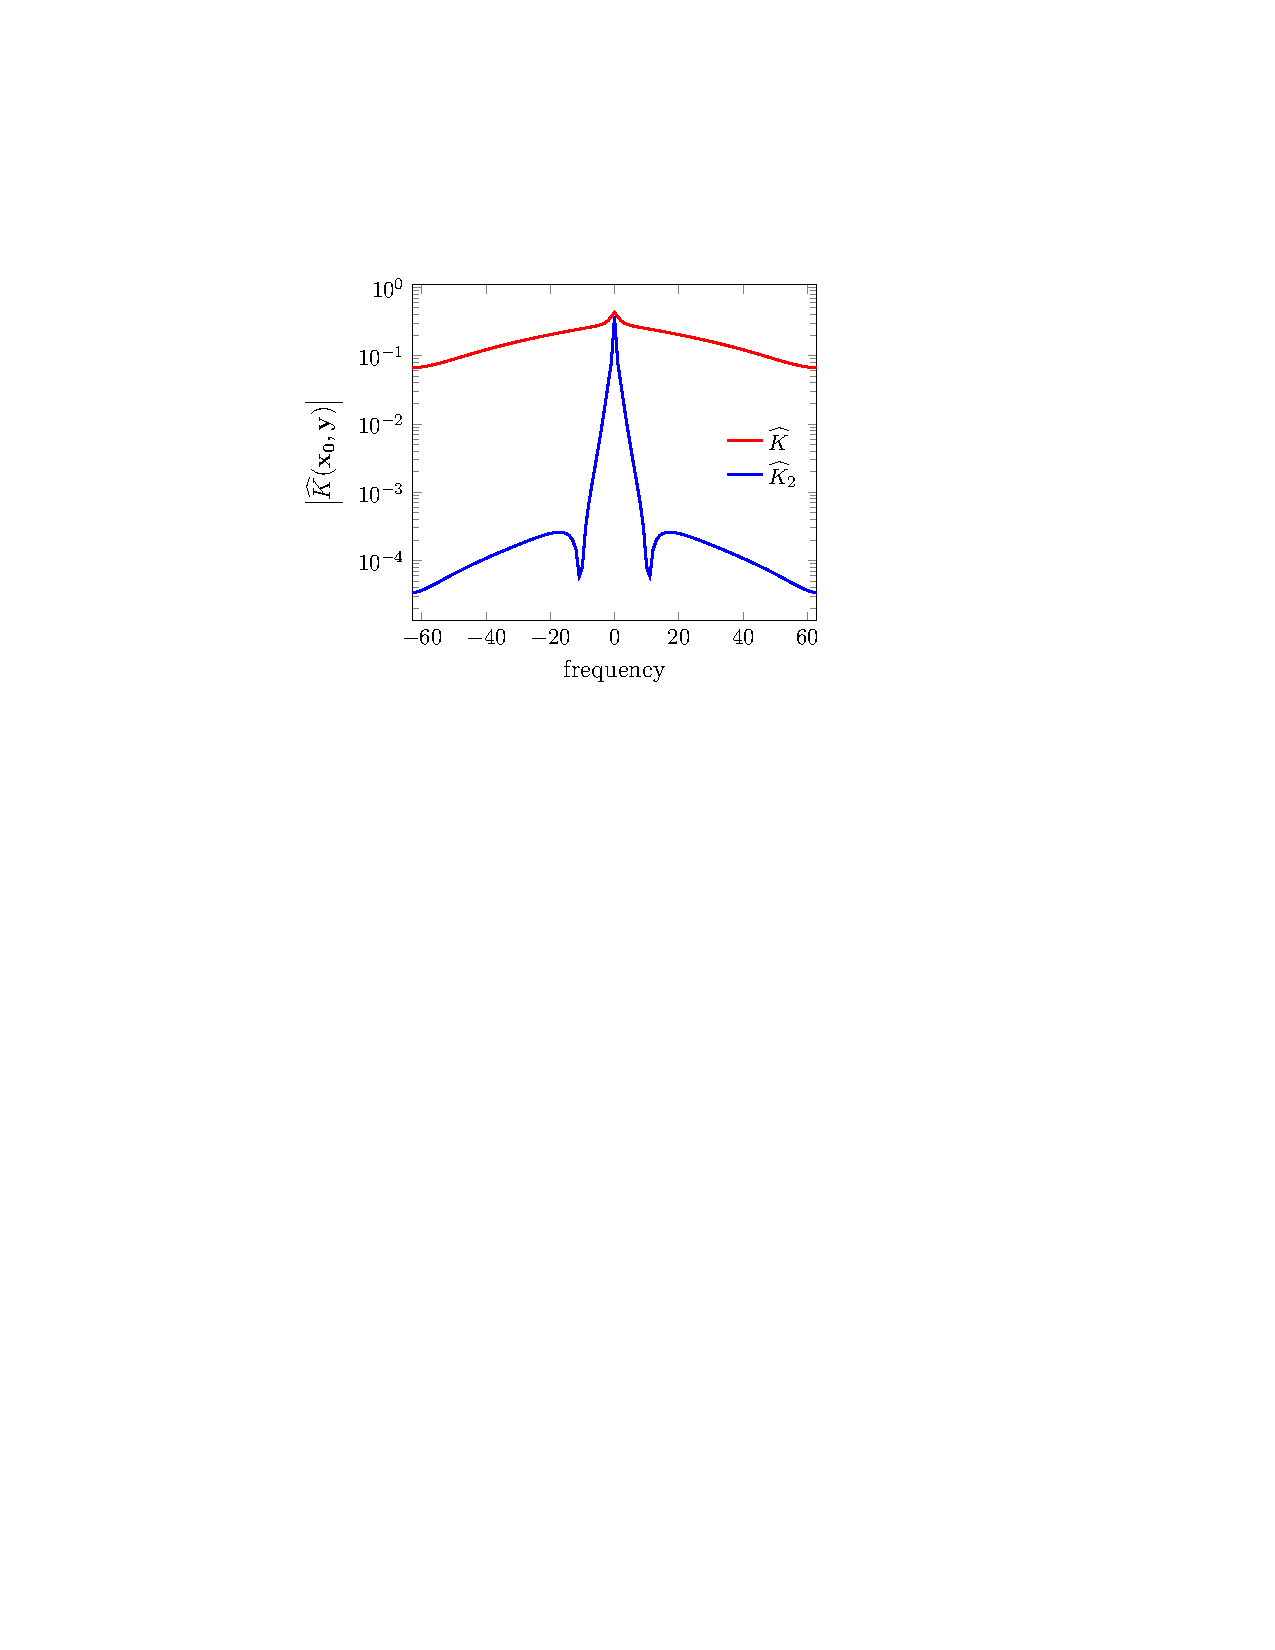
\includegraphics[width=3.0in]{figures/integrands}}
\vspace*{-10pt}
\caption{{\footnotesize The Fourier modes of $K(x_0,y)$ and $K_2(x_0,y)$
  where $\|x_0\| = 0.99$ and $\partial\Omega$ is the unit circle. The
  trapezoid rule applied to the red integrand has large amounts of
  error. However, the trapezoid rule is much more accurate when applied
  to the blue integrand. Since the difference between the red and blue
  curves can be accurately computed with the barycentric quadrature
  rule, the error of this quadrature rule applied to the screened
  Laplace layer potential will be uniformly bounded in $\Omega$.}}
\label{fig:integrands}
\end{wrapfigure}
Nearly touching bodies is ubiquitous in self-assembly of amphiphilic
particles, and such near-contact results in nearly-singular integrands
in both two and three dimensions. Quadrature methods to address such
integrands has received a lot of attention in two and three
dimensions~\cite{alpert, kapur, sidi, duffy, bruno1, bruno2, davis_1984,
graglia_2008, hackbusch_sauter_1994, jarvenpaa_2003, khayat_2005,
schwab_1992, ying_2006, beale1, beale2, goodman_1990, haroldson_1998,
lowengrub_1993, schwab_1992, ggq1, ggq2, ggq3, helsing_2008a,
helsing_integral_2009, helsing_tutorial_2012, klockner2013jcp, qbx2,
wala2019jcp, af2018sisc, siegel2018jcp, rachh2017jcp, ding2019arxiv,
bar2014}. For two-dimensional problems, the trapezoid rule is the
workhorse for BIEs since it achieves spectral accuracy when integrands
are not nearly-singular~\cite{tre-wei2014}. To address nearly-singular
integrands of two dimensional BIEs, we will use a {\em barycentric
quadrature rule} that only requires a slight modification of the
trapezoid rule~\cite{ioa-pap-per1991}. In its current form, this method
requires the layer potential satisfy Laplace or Stokes
equations~\cite{bar-wu-vee2015, chi-moo-qua2020}. The PIs will extend
this quadrature rule so that it can be applied to the screened Laplace
equation. This will be done by recognizing that the fundamental solution
of the screened Laplace equation can be decomposed as $K(x,y) = K_1(x,y)
+ K_2(x,y)$, where $K_1(x,y) = -\log\|x - y\|$ and $K_2(x,y) = K(x,y) +
\log\|x - y\|$. Using this decomposition, the layer potential involving
$K_1(x,y)$ can be accurately computed with the barycentric quadrature
rule~\cite{ioa-pap-per1991}, and the layer potential $K_2(x,y)$ can be
accurately computed with the trapezoid rule since the kernel is bounded
for all $x$ and $y$. To proposed method is demonstrated in
Figure~\ref{fig:integrands} where the amplitude of the Fourier modes of
$K(x_0,y)$ and $K_2(x_0,y)$ are plotted. The quadrature of the trapezoid
rule is the sum of the Fourier amplitudes not captured at the
resolution.


% ----------------------------------------------------------------------
\subsubsection{Avoiding contact with adaptive time stepping and
repulsion}
\label{subsec:timeStepping}

An outstanding numerical issue when simulating the
self-assembly of amphiphilic particles in a viscous solvent is the
collision between amphiphilic particles. The hydrophobic attraction
potential drives the amphiphilic particles towards one another so to
minimize exposure to the solvent, and this leads to physical contact in
finite time. Such particle collisions in a dense rigid body suspension
is a great challenge and can be a bottleneck in large-scale simulations.
We propose two algorithms to remedy this computational
challenge---high-order adaptive time stepping and repulsion forces.

PI Quaife developed a high-order adaptive time stepping method for
hydrodynamic suspensions~\cite{qua-bir2016} and he has used it with
colleagues to investigate mixing and adhesion in
suspensions~\cite{qua-vee-you2019, kab-qua-bir2017}. The method requires
both a single-step high-order time stepping method and a computationally
cheap estimate of the error. We plan to use a spectral deferred
correction method~\cite{dut-gre-rok2000} since it can be used
iteratively to increase the order of accuracy. To estimate the error,
instead of using an embedded Runge-Kutta method or step-doubling, we
will compute the total force and torque of the system which is
computationally cheap and should be zero. The PIs experience is that
error estimates based on physical constraints such as force- and
torque-free conditions appropriately adjusts the time step size so that
the dynamics are adequately resolved.

Our previous work avoids contact by including a Leonard-Jones potential
in the body forces~\cite{Fu2018_SIAM}. Such steep steric interaction at
short ranges introduces great numerical stiffness that limit the time
step size. To remove this stiffness, we will use a geometry-based
contact method~\cite{har-pon-sor-zor2011}, and this method has been
applied to vesicle suspensions~\cite{lu-rah-zor2017} and rigid body
suspensions in two dimensions~\cite{bys-sha-qua2020} and
three dimensions~\cite{Yan2019}. These methods determine repulsion
force by solving a non-linear complementarity problem with a geometric
constraint that the configuration is non-overlapping.


% ----------------------------------------------------------------------
\subsubsection{Fluctuating hydrodynamics}
\label{subsec:fluctuating}
Once algorithms that address quadrature, adaptive time stepping, and
contact are implemented, we will embark on incorporating fluctuating
hydrodynamics~\cite{Bao17,Bao18} which are important even at scales of
the some amphiphilic particles.

\todo[inline]{Using DLP formulation for fluctuating hydrodynamics so
that we have a second-kind BIE}
%\textcolor{red}{
%Once the collision-resolution algorithm is implemented, we will check
%the computing performance first before we embark on incorporating
%fluctuating hydrodynamics~\cite{Bao17,Bao18}, which might be important
%even at the scales of the amphiphilic particle size in some cases. We
%propose to extend the high-order time-integration scheme for a
%stochastic differential equation~\cite{fu2015pre} to this system.
%}




